\chapter{Results and Discussion}
\label{ch:results}

This chapter first places the adapters against full fine-tuning and the linear probe, then answers the
four research questions in turn, and closes with deployment cost, a comparison with published few-shot
results, and the limitations of the study. All numbers are means over three training seeds, each
evaluated on the same 600 test episodes. The complete per-configuration tables are in
\cref{app:tables}.

\paragraph{A note on one corrected run.} While completing the analysis we found that one of the 120
result files (CIFAR-FS, 5-shot, MobileNetV3-Small, LoRA, evidential, seed 42) had been written by a
20-episode smoke test rather than the full 600-episode evaluation. The run was retrained and evaluated
properly; the retrained model reproduced the smoke test's numbers on the first 20 episodes exactly. All
numbers in this thesis use the corrected run. The correction changes that configuration's accuracy from
86.97\% to 87.52\% and moves the RQ1 variance shares by at most 0.7 percentage points; no conclusion
changes.

\section{Parameter Efficiency}
\label{sec:efficiency}

\Cref{fig:efficiency} compares the parallel bottleneck adapter with the two baselines on CIFAR-FS and
ResNet-18. At 5-shot, the 31,744-parameter adapter reaches 91.44\% accuracy against 90.47\% for full
fine-tuning, which trains $352\times$ more parameters (11,176,512), and 87.41\% for the linear probe,
which trains none. With the evidential head the picture is the same (91.58\% against 88.82\% and
87.41\%).

\begin{figure}[H]
\centering
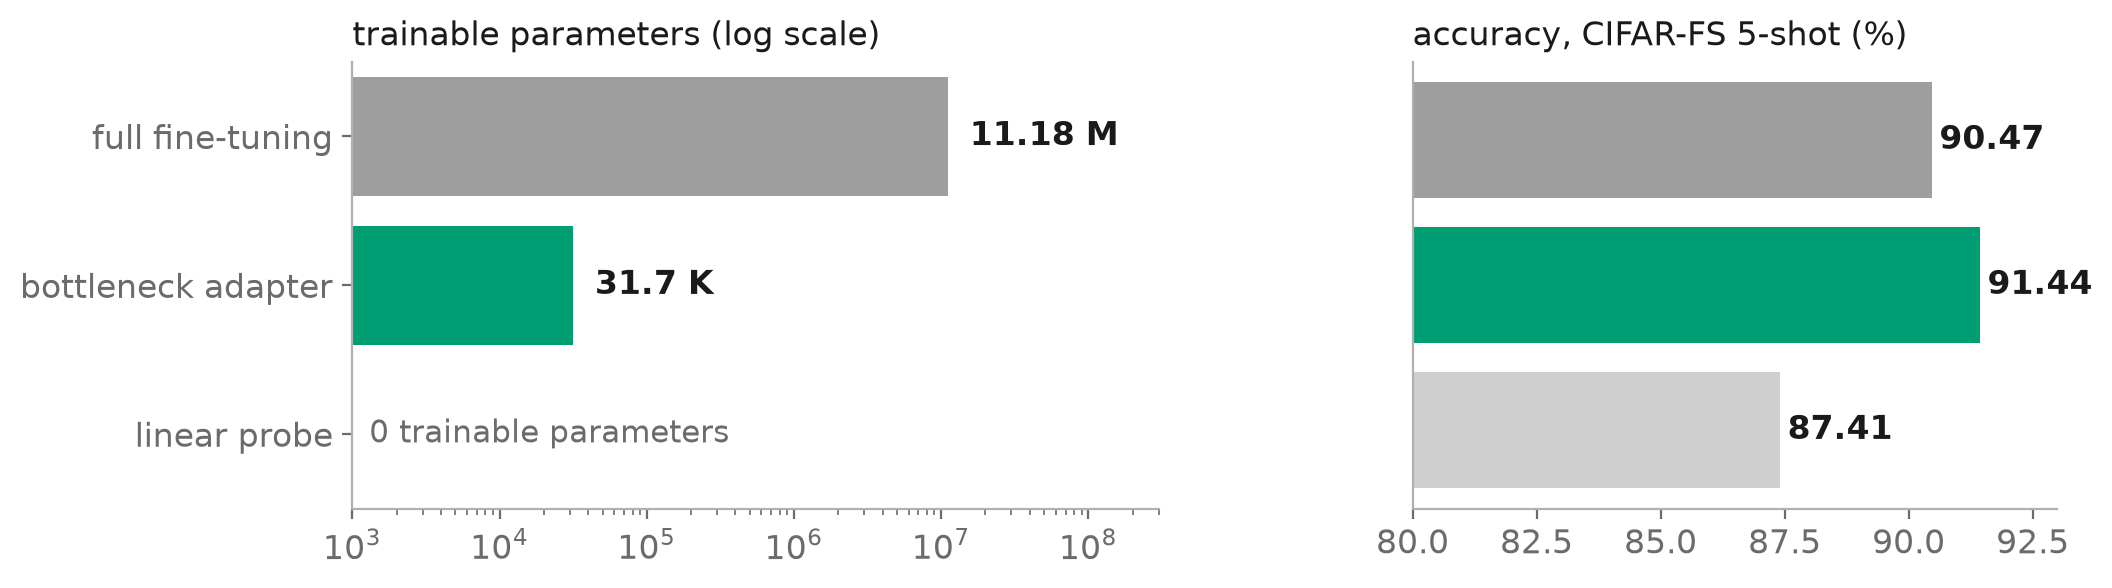
\includegraphics[width=\textwidth]{D2_parameter_efficiency_bars.png}
\caption{Trainable parameters (left, log scale) and accuracy (right) of full fine-tuning, the parallel
bottleneck adapter and the linear probe on CIFAR-FS 5-shot with ResNet-18 (softmax head).}
\label{fig:efficiency}
\end{figure}

Two qualifications matter. First, the advantage does not hold at 1-shot: there, full fine-tuning
reaches 81.14\% against 78.57\% for the adapter (80.36\% against 79.19\% with the evidential head). The
adapter comes close to full fine-tuning at 1-shot and beats it at 5-shot, but it does not dominate it. Second,
not every adapter beats the linear probe. At 5-shot on ResNet-18, LoRA reaches only 86.25\% (softmax) and
83.33\% (evidential), below the probe's 87.41\%. Adaptation pays off for the bottleneck adapter in every
setting, but not automatically for any adapter. The linear probe being a strong reference agrees with
Chen et al.'s observation that simple baselines are competitive in few-shot
classification~\cite{chen2019closer}.

The two baselines have no randomly initialised weights, and the training episodes do not depend on the
seed, so their three runs are identical. Comparisons against them therefore rest on one effective run.

\section{RQ1: What Explains Each Outcome?}
\label{sec:rq1}

We computed the share of variance ($\eta^2$) that each factor explains for each outcome, using all 96
runs of the balanced $2^5$ factorial (32 configurations $\times$ 3 seeds; the baselines are excluded).
Using individual runs rather than seed means keeps a genuine residual term. For OOD detection we use
SVHN as the far-OOD outcome and TinyImageNet as the near-OOD outcome, because TinyImageNet does not share
classes with the validation split.

\begin{table}[H]
\centering
\caption{Share of variance explained by each factor ($\eta^2$, \%), 96 runs. Bold marks the dominant
factor where one exists.}
\label{tab:eta}
\begin{adjustbox}{max width=\textwidth}
\begin{tabular}{@{}lrrrrrr@{}}
\toprule
Outcome & Dataset & Shots & Backbone & Adapter & Head & Residual \\
\midrule
Accuracy & 1.69 & \textbf{76.31} & 3.82 & 8.98 & 0.16 & 9.04 \\
ECE & 1.98 & 2.16 & 4.56 & 0.65 & \textbf{82.97} & 7.68 \\
OOD AUROC, far (SVHN) & 1.23 & 22.59 & 11.71 & 1.79 & 38.93 & 23.75 \\
OOD AUROC, near (TinyImageNet) & 1.54 & 43.30 & 0.55 & 21.68 & 21.44 & 11.49 \\
\bottomrule
\end{tabular}
\end{adjustbox}
\end{table}

\begin{figure}[H]
\centering
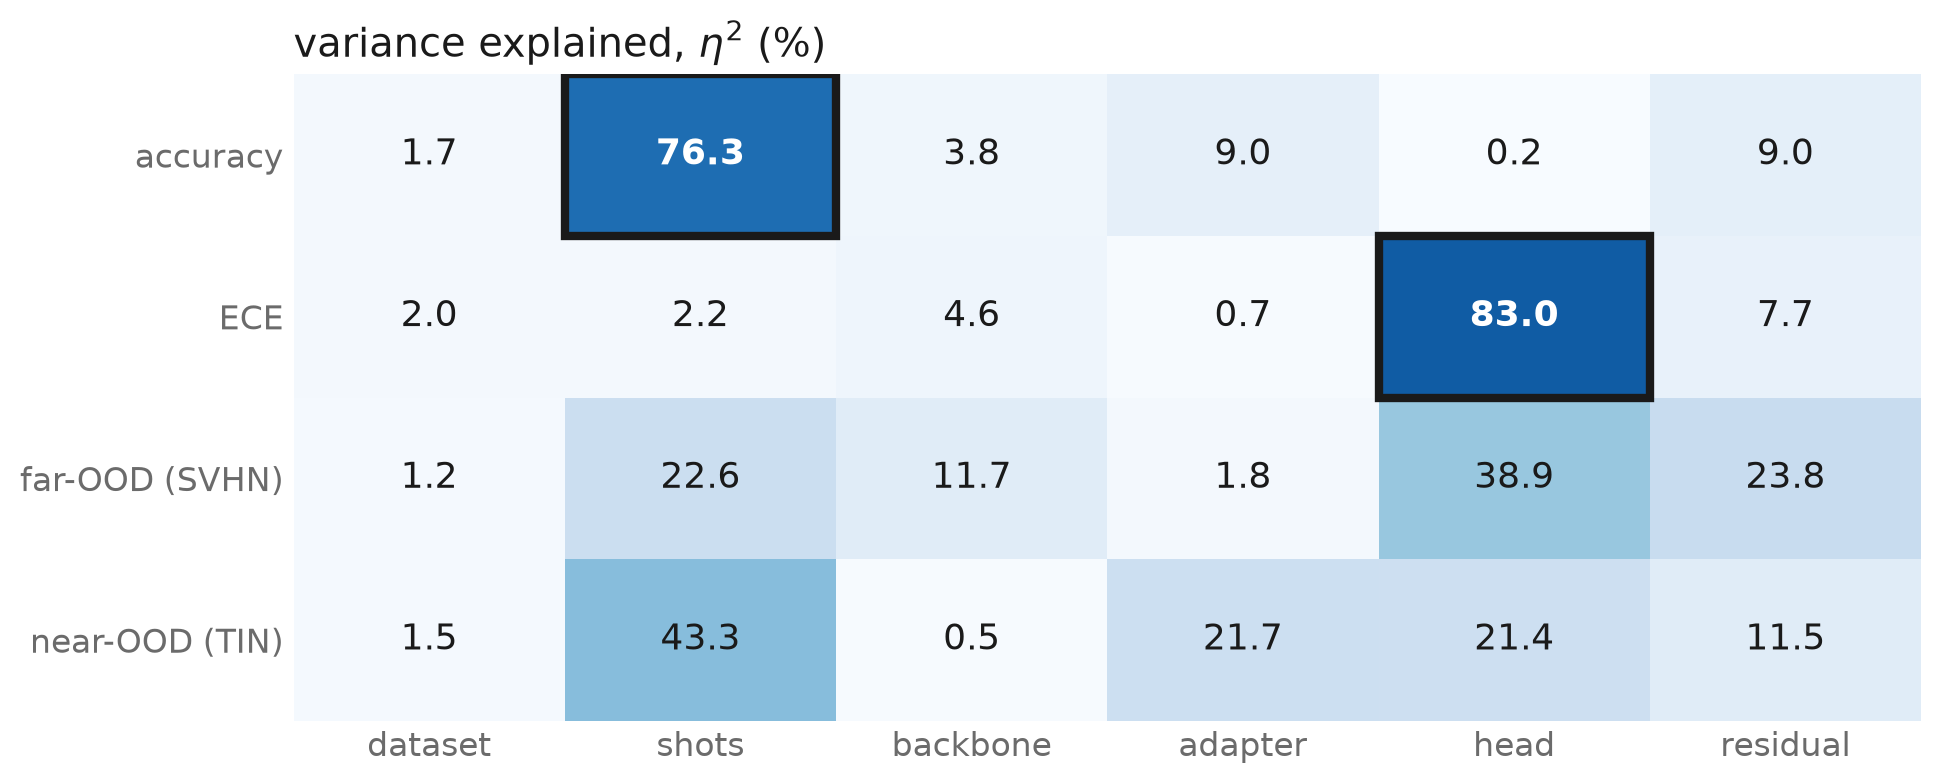
\includegraphics[width=0.9\textwidth]{F11_main_effects_heatmap.png}
\caption{The variance shares of \cref{tab:eta} as a heatmap. Accuracy is dominated by shot count and
calibration by the head; neither OOD outcome has a single dominant factor.}
\label{fig:heatmap}
\end{figure}

\paragraph{Accuracy and calibration are governed by different factors.} Shot count explains 76\% of the
variance in accuracy, and adapter type is a distant second at 9\%. The head explains 83\% of the
variance in calibration but only 0.16\% of the variance in accuracy. In practice the head changes how
confident the model is while leaving what it predicts almost untouched: across the 20 matched pairs that
differ only in the head, the evidential head is more accurate in 7 and the softmax head in 13, and no
difference exceeds 0.7 percentage points in the evidential head's favour.

\paragraph{The evidential head is worse calibrated in every case.} In all 20 matched pairs, the evidential
head has a higher pooled ECE than the softmax head, by a factor of 1.4 to 9.1, and a higher ECE than the
temperature-scaled softmax by a factor of 5.3 to 51. \Cref{tab:ece-head} shows the ResNet-18 bottleneck
configurations as an example. The gap does not shrink with more data: at 5-shot it is as large as at
1-shot. The reliability diagrams we inspected (ResNet-18 with the bottleneck adapter) show that the evidential
head is \emph{under}confident (accuracy higher than confidence in every bin), so its problem is the opposite of the overconfidence
usually reported for softmax networks.

\begin{table}[H]
\centering
\caption{Pooled ECE of the ResNet-18 bottleneck configurations. Lower is better.}
\label{tab:ece-head}
\begin{adjustbox}{max width=\textwidth}
\begin{tabular}{@{}llrrr@{}}
\toprule
Dataset & Shots & Evidential & Softmax & Softmax + temperature scaling \\
\midrule
CIFAR-FS & 1 & 0.2765 & 0.0560 & 0.0297 \\
CIFAR-FS & 5 & 0.3010 & 0.0670 & 0.0152 \\
MiniImageNet & 1 & 0.3073 & 0.1012 & 0.0073 \\
MiniImageNet & 5 & 0.2938 & 0.0850 & 0.0057 \\
\bottomrule
\end{tabular}
\end{adjustbox}
\end{table}

This negative result does not contradict the evidential literature so much as mark a boundary. BEL and
BayesAdapter report calibration improvements from evidential or Bayesian
modelling~\cite{linghu2022bel,moralesalvarez2026bayesadapter}, but with a meta-trained backbone or a
larger adaptation budget than ours. With a frozen backbone and an adapter of a few thousand parameters
we see the opposite.

\paragraph{Calibration and OOD detection are not in tension once the head is fixed.} Across the 40
configurations, the rank correlation between ECE and OOD AUROC is positive (Spearman $\rho = 0.43$ for
SVHN, $0.48$ for TinyImageNet), which would suggest that worse-calibrated models detect OOD inputs better.
Within each head the correlation drops to $0.15$/$0.20$ (evidential) and $0.26$/$0.24$ (softmax). The
apparent trade-off is almost entirely a head effect: the evidential head is both worse calibrated and,
with its native vacuity score, a better OOD detector. RQ2 shows where the second part comes from.

\paragraph{Interactions.} Adding the ten two-way interactions to the model lowers the residual from 9.0\%
to 1.3\% for accuracy and from 7.7\% to 2.0\% for ECE. For calibration the largest interaction is
backbone $\times$ adapter (3.23\%, 95\% bootstrap interval 2.49--4.05\%), while the same interaction is
negligible for accuracy (0.8\%) and for both OOD outcomes (0.2\% and 0.0\%). In other words, which adapter
calibrates better depends on the backbone, but which adapter is more accurate does not. RQ3 tests this
directly.

\section{RQ2: Training Objective or Scoring Rule?}
\label{sec:rq2}

\paragraph{The native comparison.} In the grid, each evidential model is scored with vacuity and each
softmax model with MSP, TS-MSP and energy. Comparing each evidential model's vacuity with its softmax
sibling's scores, over the two far-OOD sets and the two near-OOD sets of the 20 matched pairs (40
comparisons each), gives:

\begin{table}[H]
\centering
\caption{Vacuity (evidential models) against the softmax models' scores. Wins out of 40 comparisons per
OOD type, and mean AUROC difference.}
\label{tab:vacuity-wins}
\begin{adjustbox}{max width=\textwidth}
\begin{tabular}{@{}lrrrr@{}}
\toprule
& \multicolumn{2}{c}{Far-OOD} & \multicolumn{2}{c}{Near-OOD} \\
\cmidrule(lr){2-3}\cmidrule(lr){4-5}
Vacuity vs. & Wins & Mean $\Delta$AUROC & Wins & Mean $\Delta$AUROC \\
\midrule
MSP & 38/40 & $+0.111$ & 37/40 & $+0.053$ \\
TS-MSP & 38/40 & $+0.127$ & 38/40 & $+0.067$ \\
Energy & 10/40 & $-0.022$ & 14/40 & $-0.007$ \\
\bottomrule
\end{tabular}
\end{adjustbox}
\end{table}

Vacuity is clearly better than the probability-based scores, but the parameter-free energy score beats it
in about 70\% of comparisons. This overturns an earlier result from a single configuration in this
project, where vacuity had looked roughly on par with energy. It also raises the question RQ2 asks:
because the evidential models were scored only with vacuity and the softmax models only with the other
scores, these comparisons change the training objective and the score together. ``Energy beats vacuity''
could mean that energy is a better score, or that softmax training produces logits that any score
separates better.

\paragraph{Separating objective and score.} We therefore computed all four scores on all 120 models and
decomposed the AUROC variance over the full $2 \times 4$ (objective $\times$ score) design, with 960
observations per OOD type (120 models $\times$ 4 scores $\times$ 2 OOD sets).

\begin{table}[H]
\centering
\caption{Share of OOD-AUROC variance explained by the scoring rule and by the training objective.}
\label{tab:rq2}
\begin{adjustbox}{max width=\textwidth}
\begin{tabular}{@{}lrr@{}}
\toprule
OOD type & Scoring rule $\eta^2$ & Training objective $\eta^2$ \\
\midrule
Far-OOD & 42.69\% & 0.17\% \\
Near-OOD & 14.72\% & 0.63\% \\
\bottomrule
\end{tabular}
\end{adjustbox}
\end{table}

\begin{table}[H]
\centering
\caption{Mean OOD AUROC by score and training objective. Each cell averages 60 models over the two OOD
sets of its type.}
\label{tab:rq2-means}
\begin{adjustbox}{max width=\textwidth}
\begin{tabular}{@{}llrrrr@{}}
\toprule
OOD type & Trained as & MSP & TS-MSP & Energy & Vacuity \\
\midrule
Far & evidential & 0.799 & 0.787 & 0.919 & 0.913 \\
Far & softmax & 0.801 & 0.785 & 0.934 & 0.931 \\
Near & evidential & 0.792 & 0.781 & 0.841 & 0.835 \\
Near & softmax & 0.777 & 0.763 & 0.837 & 0.823 \\
\bottomrule
\end{tabular}
\end{adjustbox}
\end{table}

\begin{figure}[H]
\centering
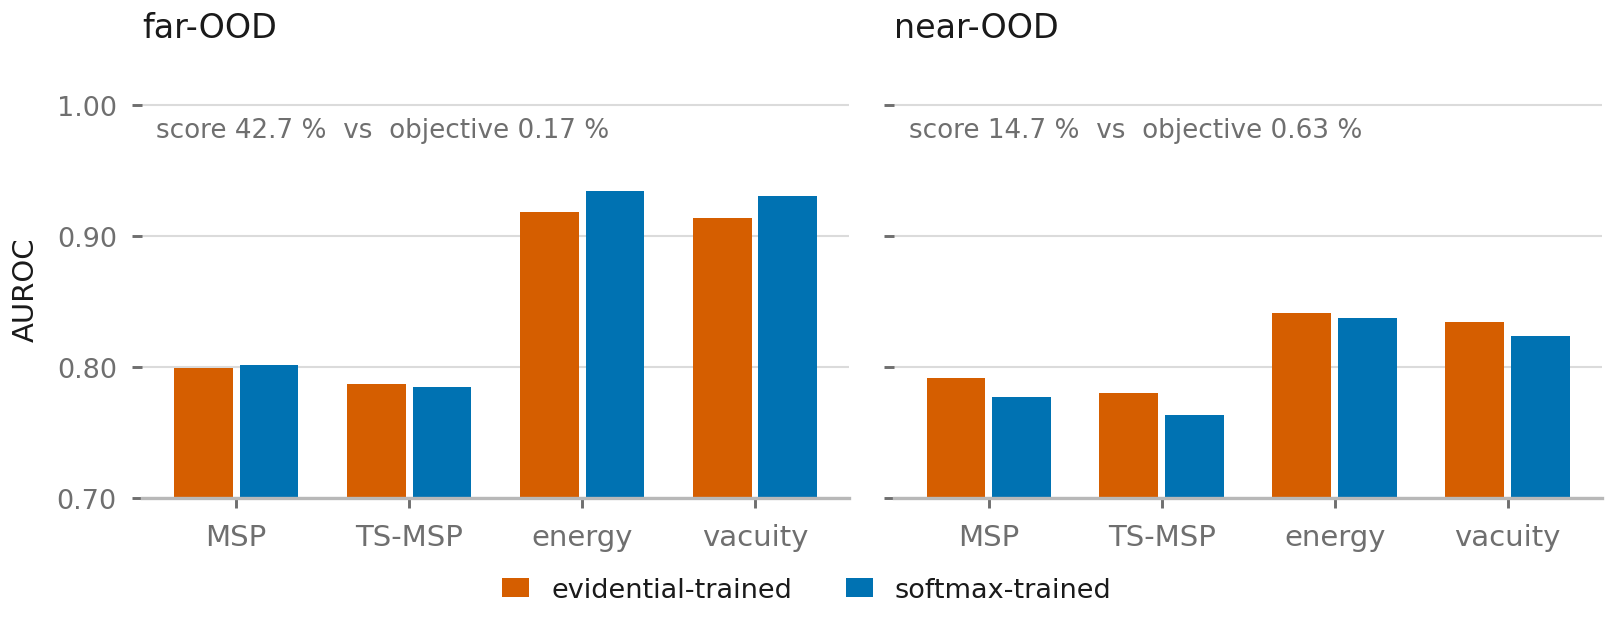
\includegraphics[width=\textwidth]{F12_ood_score_vs_objective.png}
\caption{Mean OOD AUROC by score and by training objective. The same score gives nearly the same AUROC
whichever objective trained the model; the differences between scores are much larger.}
\label{fig:rq2}
\end{figure}

The scoring rule matters far more than the training objective. On far-OOD it explains 42.7\% of the
variance against 0.17\% for the objective; on near-OOD, 14.7\% against 0.63\%. The same score gives almost
the same AUROC whichever objective produced the logits: energy reaches 0.919 on evidential-trained models
and 0.934 on softmax-trained ones, while MSP stays near 0.80 under both. The OOD advantage the evidential
head seemed to offer comes from reading the logits through a score that looks at the absolute strength of
the match (vacuity or energy) rather than at relative class probabilities (MSP), not from evidential
training. This agrees with the theoretical result that softmax is a special case of an evidential
classifier~\cite{hayta2026plugin}. We report the variance shares rather than their ratio: because the
objective's share is close to zero, the ratio is unstable and changed from about $160\times$ to about
$250\times$ when the last 21 models were added to the analysis, while the shares themselves barely
moved.

Related work is close but not identical. Gen{\c{c}} et al.~\cite{genc2026objectives} name the
objective/score confound as an open problem but study no evidential objective, and Krumpl et
al.~\cite{krumpl2026onemodel} cross training methods with detectors at a much larger scale without
evidential models. The part we did not find elsewhere is the cross-application of energy to
Dirichlet-trained logits and the finding that it performs almost the same as on softmax-trained logits.

\section{RQ3: Architecture or Budget?}
\label{sec:rq3}

RQ1 found that the adapter explains only 0.65\% of calibration variance in total. RQ3 asks a different
question: when two adapters are compared directly, which property predicts the winner? A factor can
contribute little total variance and still point in a very consistent direction.

\subsection{Evidence from the grid}

The grid contains 16 matched bottleneck-versus-LoRA pairs (2 datasets $\times$ 2 shot counts $\times$ 2
backbones $\times$ 2 heads), identical except for the adapter.

\begin{table}[H]
\centering
\caption{The 16 matched pairs. Accuracy in \%, gap = bottleneck minus LoRA; better-calibrated adapter in bold.}
\label{tab:pairs}
\small
\begin{adjustbox}{max width=\textwidth}
\begin{tabular}{@{}lllrrrrr@{}}
\toprule
Dataset & Shots & Backbone / head & Acc.\ btl & Acc.\ LoRA & Gap & ECE btl & ECE LoRA \\
\midrule
CIFAR-FS & 1 & ResNet-18 / softmax & 78.57 & 75.44 & $+3.12$ & \textbf{0.056} & 0.097 \\
CIFAR-FS & 1 & ResNet-18 / evid. & 79.19 & 73.76 & $+5.43$ & \textbf{0.277} & 0.297 \\
CIFAR-FS & 5 & ResNet-18 / softmax & 91.44 & 86.25 & $+5.19$ & \textbf{0.067} & 0.102 \\
CIFAR-FS & 5 & ResNet-18 / evid. & 91.58 & 83.33 & $+8.26$ & \textbf{0.301} & 0.329 \\
MiniImageNet & 1 & ResNet-18 / softmax & 85.03 & 80.29 & $+4.75$ & \textbf{0.101} & 0.175 \\
MiniImageNet & 1 & ResNet-18 / evid. & 84.81 & 79.16 & $+5.65$ & \textbf{0.307} & 0.371 \\
MiniImageNet & 5 & ResNet-18 / softmax & 95.56 & 91.56 & $+4.00$ & \textbf{0.085} & 0.193 \\
MiniImageNet & 5 & ResNet-18 / evid. & 95.88 & 88.32 & $+7.56$ & \textbf{0.294} & 0.405 \\
\midrule
CIFAR-FS & 1 & MNv3-S / softmax & 78.80 & 75.43 & $+3.37$ & 0.050 & \textbf{0.029} \\
CIFAR-FS & 1 & MNv3-S / evid. & 78.88 & 74.03 & $+4.85$ & 0.254 & \textbf{0.216} \\
CIFAR-FS & 5 & MNv3-S / softmax & 90.74 & 88.05 & $+2.70$ & 0.070 & \textbf{0.062} \\
CIFAR-FS & 5 & MNv3-S / evid. & 90.24 & 87.52 & $+2.72$ & 0.304 & \textbf{0.293} \\
MiniImageNet & 1 & MNv3-S / softmax & 74.92 & 72.45 & $+2.47$ & 0.065 & \textbf{0.024} \\
MiniImageNet & 1 & MNv3-S / evid. & 75.61 & 72.48 & $+3.14$ & 0.253 & \textbf{0.219} \\
MiniImageNet & 5 & MNv3-S / softmax & 90.10 & 87.96 & $+2.13$ & 0.111 & \textbf{0.096} \\
MiniImageNet & 5 & MNv3-S / evid. & 90.64 & 87.96 & $+2.68$ & 0.318 & \textbf{0.305} \\
\bottomrule
\end{tabular}
\end{adjustbox}
\end{table}

\begin{figure}[H]
\centering
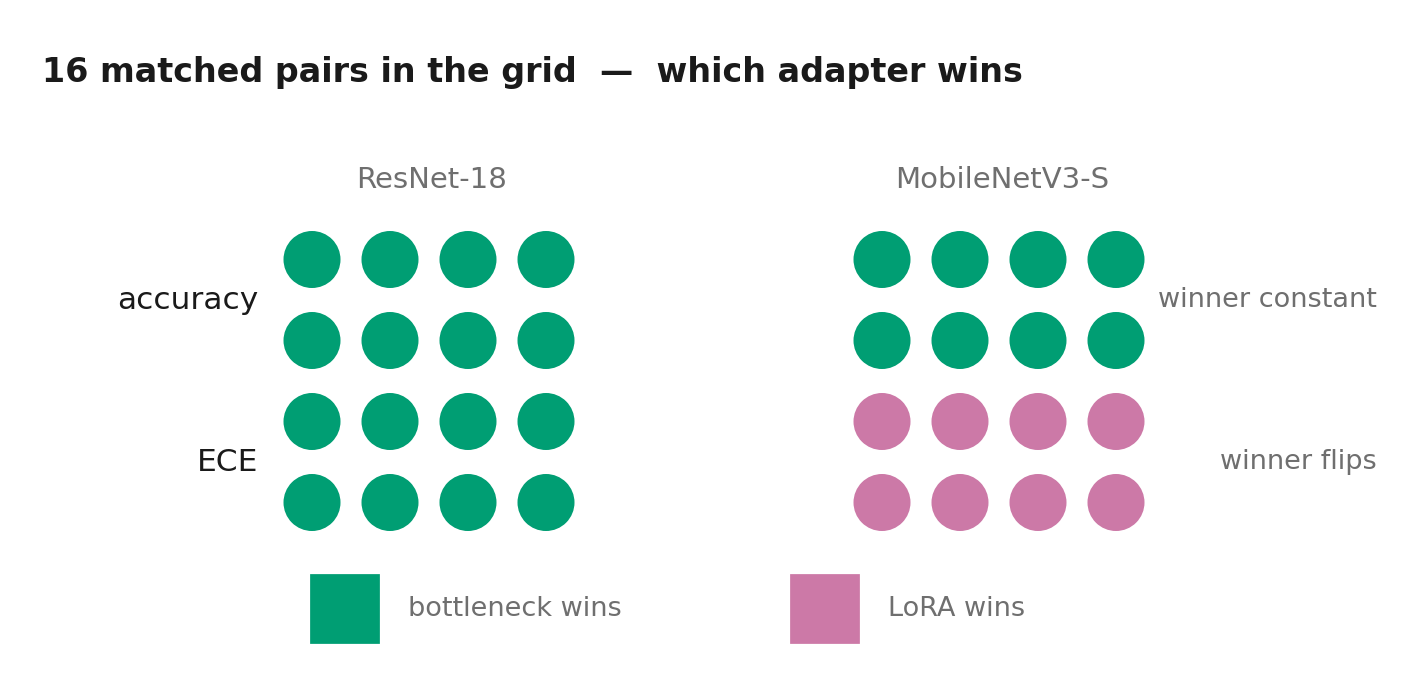
\includegraphics[width=0.75\textwidth]{F13_matched_pairs_deltas.png}
\caption{Which adapter wins each of the 16 pairs. The accuracy winner never changes; the calibration winner
changes with the backbone.}
\label{fig:pairs}
\end{figure}

Two facts stand out (\cref{tab:pairs,fig:pairs}).
\begin{enumerate}
\item \textbf{The accuracy winner does not change when the size ordering reverses.} The bottleneck adapter
is more accurate in all 16 pairs, by 2.1 to 8.3 percentage points, both on ResNet-18, where it has
$2.58\times$ more parameters than LoRA, and on MobileNetV3-Small, where it has $1.55\times$ fewer. Size
cannot explain this, so accuracy follows architecture. The bottleneck also gives the better near-OOD
AUROC in all 16 pairs. For far-OOD (SVHN) it wins only 11 of 16, so we make no claim there.
\item \textbf{The calibration winner flips with the backbone.} The bottleneck is better calibrated in all 8
ResNet-18 pairs and LoRA in all 8 MobileNetV3-Small pairs. The direction is very consistent (a 16-of-16
sign pattern has $p \approx 3 \times 10^{-5}$ under random directions), although the size of the
calibration gap exceeds twice the seed-to-seed spread in only 10 of the 16 pairs, all 8 MiniImageNet
pairs but only 2 of the 8 CIFAR-FS pairs.
\end{enumerate}

The second fact admits two explanations. The better-calibrated adapter is always the \emph{larger} one,
which suggests that calibration follows the parameter budget. But it is also always ``whichever adapter
suits this backbone'', because in this grid the size ordering flips exactly when the backbone changes.
The two explanations predict identical patterns here, so the grid cannot decide between them.

\subsection{The matched-budget experiment}

The pre-registered matched-budget experiment (\cref{sec:matched-design}) removes the size difference
within each backbone. If budget caused the calibration gap, the gap should collapse once the budgets are
equal. \Cref{tab:matched} gives the result for each cell, averaged over the two budget levels, and
\cref{fig:matched} compares it with the grid.

\begin{table}[H]
\centering
\caption{Matched-budget calibration results. $\Delta$ = LoRA ECE minus bottleneck ECE. Collapse ratio =
matched $|\Delta|$ divided by unmatched $|\Delta|$. Per-level numbers are in \cref{tab:matched-levels}.}
\label{tab:matched}
\small
\begin{adjustbox}{max width=\textwidth}
\begin{tabular}{@{}llrrrrrrl@{}}
\toprule
Backbone & Head & ECE btl & ECE LoRA & $\Delta$ matched & $\Delta$ grid & Ratio & $2\sigma$ & Rule fired \\
\midrule
ResNet-18 & evidential & 0.296 & 0.408 & $+0.112$ & $+0.111$ & 1.01 & 0.035 & backbone \\
ResNet-18 & softmax & 0.084 & 0.183 & $+0.099$ & $+0.108$ & 0.92 & 0.012 & backbone \\
MNv3-S & evidential & 0.317 & 0.311 & $-0.006$ & $-0.012$ & 0.50 & 0.002 & backbone \\
MNv3-S & softmax & 0.112 & 0.106 & $-0.006$ & $-0.015$ & 0.61 & 0.015 & none \\
\bottomrule
\end{tabular}
\end{adjustbox}
\end{table}

\begin{figure}[H]
\centering
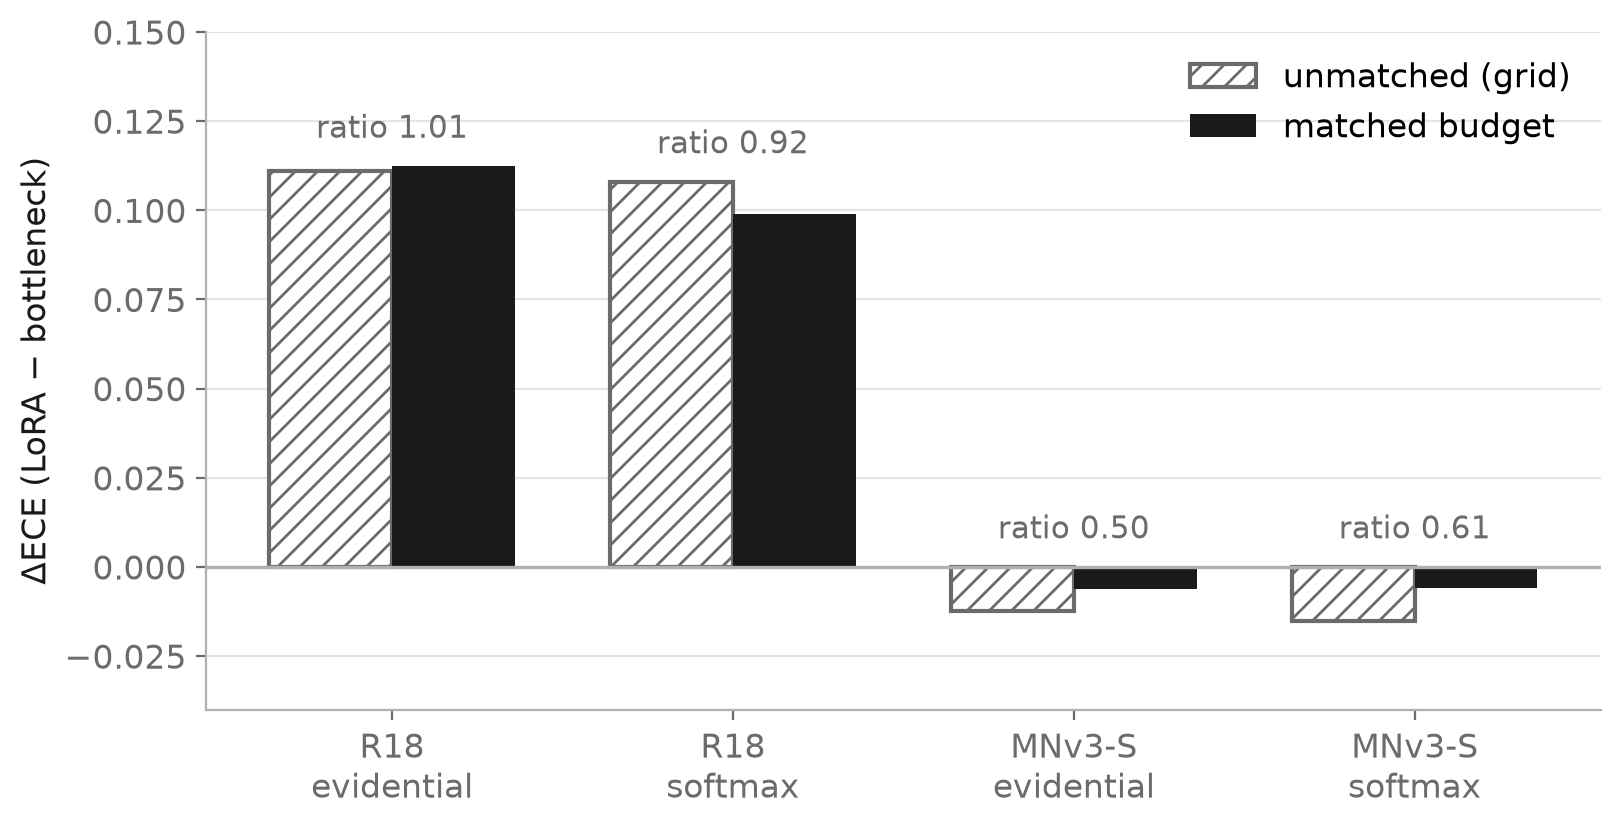
\includegraphics[width=0.85\textwidth]{F14a_matched_budget_bars.png}
\caption{$\Delta$ECE (LoRA $-$ bottleneck) in the grid (hatched) and at matched budget (solid). The labels
give the pre-registered collapse ratios. On ResNet-18 the gap is unchanged; on MobileNetV3-Small it
shrinks but keeps its sign.}
\label{fig:matched}
\end{figure}

\paragraph{Verdict.} The budget rule fired in 0 of 4 cells and the backbone rule in 3 of 4, against a
pre-set threshold of 3; the architecture rule fired in none, because the sign still differs between
backbones. The pre-registered verdict is therefore \emph{backbone}:
\begin{itemize}
\item On ResNet-18, equalising the budgets left the calibration gap where it was (collapse ratios 1.01 and
0.92). At the high budget, for example, the softmax bottleneck has ECE 0.085 and the softmax LoRA 0.173
with almost the same number of parameters. A gap caused by the budget difference should have
disappeared with it.
\item On MobileNetV3-Small, the gap roughly halved (ratios 0.50 and 0.61) but kept its sign. Budget
therefore affects the size of the gap there, but not its direction.
\item The softmax MobileNetV3-Small cell fired no rule: its matched gap ($-0.006$) is smaller than its
noise ($2\sigma = 0.015$), and its two budget levels even disagree in sign.
\item The two backbones are far from symmetric. The ResNet-18 gap (about 0.10) is roughly fifteen times the
MobileNetV3-Small gap (about 0.006), so most of the evidence comes from ResNet-18.
\end{itemize}

\paragraph{The architecture half survives.} At matched budget the bottleneck is still more accurate in
all 8 comparisons and still gives the better near-OOD AUROC in all 8, every time by more than $2\sigma$.
Its accuracy lead ranges from 1.4 points (MobileNetV3-Small, softmax, low budget) to 8.6 points
(ResNet-18, evidential, high budget), and none of the accuracy gaps collapsed (ratios 0.68--1.22). Even
LoRA at rank 41, with the same 31.5K parameters as the bottleneck on ResNet-18, stays 5.8 to 8.6 points
behind. Far-OOD again shows no clear pattern (bottleneck wins 5 of 8).

\paragraph{Answer to RQ3.} Accuracy and near-OOD detection follow adapter architecture, whichever adapter
has more parameters. Calibration follows neither architecture nor budget cleanly: the better-calibrated
adapter depends on the backbone. The reading suggested by the grid alone, that calibration follows the
parameter budget, is not supported. The base-grid interaction analysis points the same way: backbone
$\times$ adapter is the largest two-way interaction for ECE and negligible for accuracy and OOD detection
(\cref{sec:rq1}).

Two caveats apply. ``Architecture'' here means each adapter as implemented: the bottleneck differs from
LoRA in its non-linearity, its placement in four stages instead of one layer, and in adding a branch
instead of changing a weight, and we do not separate these. And with only two backbones we cannot say
which property of the backbone is responsible; depth, width, normalisation, the inverted-residual block
and the scale of the features at the adapter sites all differ between them.

We found no prior work that separates adapter architecture from parameter budget by outcome. The usual
practice in PEFT studies is to compare adapters at equal budgets; Wang et al.~\cite{wang2026cptensor}
study the accuracy-versus-budget curve at a finer resolution but measure accuracy only.

\section{RQ4: Repairing Evidential Calibration}
\label{sec:rq4}

For each of the 60 evidential models we refitted only the scale $a$ and bias $b$ on the validation
episodes, keeping everything else fixed (\cref{sec:refit}).

\begin{figure}[H]
\centering
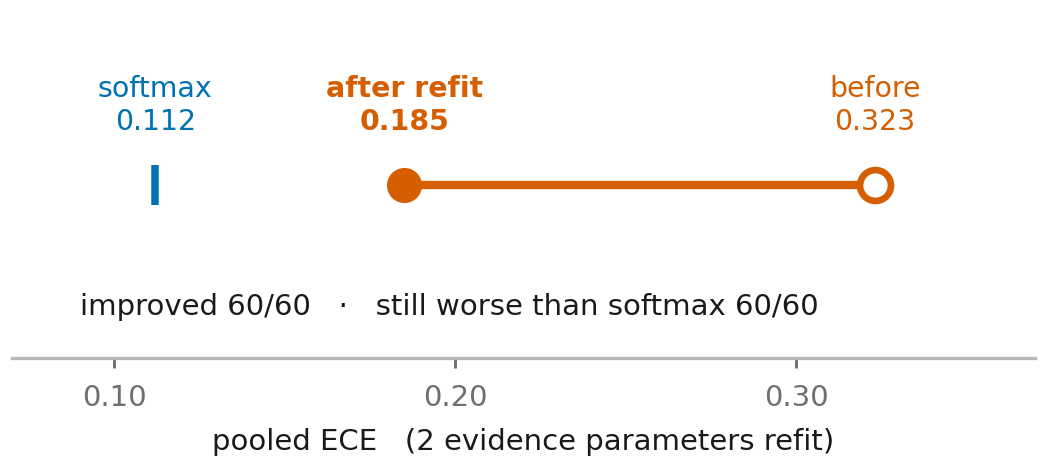
\includegraphics[width=0.8\textwidth]{F15a_ece_before_after_dumbbell.png}
\caption{Mean pooled ECE of the 60 evidential models before and after the refit, against plain softmax
applied to the same logits.}
\label{fig:refit-ece}
\end{figure}

\paragraph{Calibration improves in every model.} The refit lowers pooled ECE in 60 of 60 models, from a
mean of 0.323 to 0.185, with improvements between 0.10 and 0.18 per model. The refitted scale is much
larger than the one learned in training: 3.6 to 14.5 (median 9.0) against 1.5 to 4.5 (median 2.9), with
the bias moving from $-9.3 \ldots -5.6$ to $-26.5 \ldots -8.1$. A larger scale makes evidence grow faster
once a similarity passes the threshold, which sharpens the predictions; this is consistent with the
underconfidence seen in the reliability diagrams. Training the two parameters jointly with the adapter,
under the evidential loss, simply leaves them far from the point that minimises the validation NLL.
Accuracy is essentially unchanged (it moves by at most 0.04 percentage points in any model), as expected
from a refit that keeps the scale positive and so preserves the order of the logits.

\paragraph{It narrows the gap but does not close it.} Even after the refit, the evidential readout is
worse calibrated than a plain softmax over the \emph{same} logits in 60 of 60 models (mean ECE 0.185
against 0.112, on average $2.2\times$ higher, between $1.07\times$ and $5.8\times$), and far worse than the
temperature-scaled softmax (mean ECE 0.023, on average $13.6\times$ higher). A possible reason, which we did
not test, is that bounded cosine logits together with the ``$+1$'' prior on every class limit how much of
the Dirichlet mass the top class can hold.

\paragraph{OOD ranking mostly survives.} Comparing vacuity AUROC before and after the refit for 60 models
and four OOD sets gives 240 comparisons (\cref{fig:refit-ood}). In 192 of them (80\%) the AUROC did not
drop by more than 0.005: it stayed within $\pm 0.005$ in 154 and improved by more than 0.005 in 38. In the
remaining 48 it dropped by more than 0.005, at worst by 0.032 (Gaussian noise, CIFAR-FS 1-shot,
MobileNetV3-Small with LoRA). The mean change is $+0.003$. Reordering does happen, as anticipated in
\cref{sec:refit}: in the worst case the Spearman correlation between the vacuity rankings before and after
the refit is 0.87.

\begin{figure}[H]
\centering
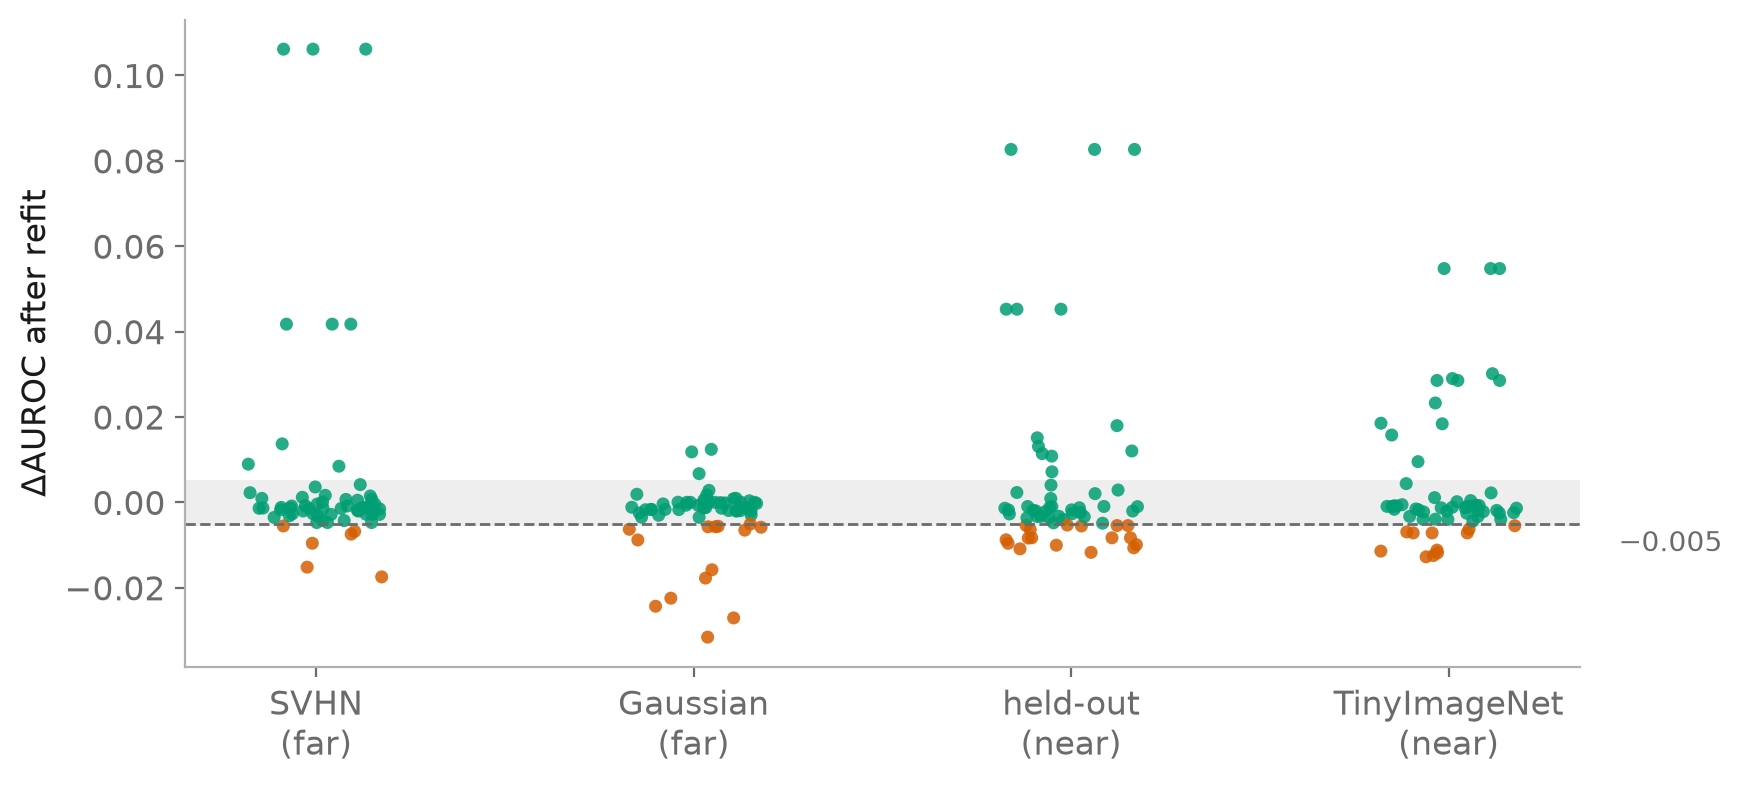
\includegraphics[width=0.85\textwidth]{F15b_delta_auroc_strip.png}
\caption{Change in vacuity AUROC after the refit for each model and OOD set (240 points). Green: did not
drop by more than 0.005. Orange: dropped by more than 0.005.}
\label{fig:refit-ood}
\end{figure}

\paragraph{Answer to RQ4.} The evidential head's calibration can be improved cheaply and reliably after
training, but not repaired: it remains worse calibrated than softmax in every model, and the refit costs a
small but real amount of OOD ranking in a fifth of the comparisons. Post-hoc calibration itself is a mature
field~\cite{guo2017calibration,kull2019dirichlet,zhao2026invlt}, and the size of the improvement is in line
with what temperature scaling and BEL report~\cite{guo2017calibration,linghu2022bel}. What we add is the
measurement of this particular two-parameter refit for an evidential prototype head, including its effect
on the OOD ranking, which existing evidential recalibration methods address by changing the model or its
training instead~\cite{carlotti2026dipedl,turacan2026invascal}.

\section{Deployment Cost}
\label{sec:deployment}

We measured inference latency for the twelve backbone, adapter and head combinations in the grid on a
single CPU thread (\cref{tab:latency,fig:latency}). The backbone dominates: with the
same adapter and head, ResNet-18 takes 62.2 ms per image and MobileNetV3-Small 12.1 ms, a $5.1\times$
difference. Switching the adapter changes latency by only 3.9\% on ResNet-18, and on MobileNetV3-Small LoRA
is 5.8\% faster than the bottleneck even though it has more parameters. The head costs nothing measurable:
the mean latency difference between evidential and softmax heads is 1.3\%, below the 5.9\% run-to-run
noise of the measurement session, and the whole uncertainty computation for a 75-query episode costs about
1\% of one image's forward pass.

\begin{table}[H]
\centering
\caption{Effect of each design choice on CPU inference latency.}
\label{tab:latency}
\begin{adjustbox}{max width=\textwidth}
\begin{tabular}{@{}lr@{}}
\toprule
Design choice & Effect on latency \\
\midrule
Backbone (ResNet-18 vs.\ MobileNetV3-Small) & $5.1\times$ \\
Adapter type & 4--6\% \\
Evidential vs.\ softmax head & about 1\%, within measurement noise \\
\bottomrule
\end{tabular}
\end{adjustbox}
\end{table}

\begin{figure}[H]
\centering
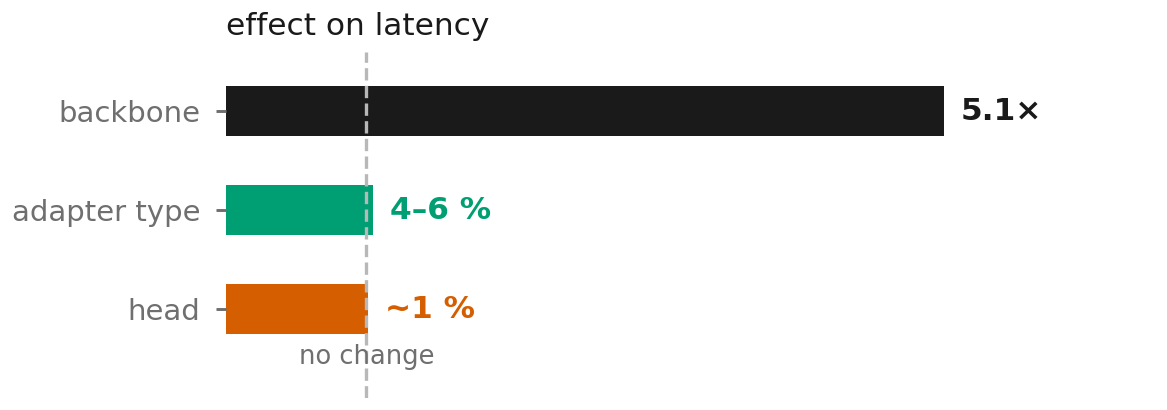
\includegraphics[width=0.75\textwidth]{D3_latency_effect_bars.png}
\caption{Effect of backbone, adapter type and head on single-thread CPU latency.}
\label{fig:latency}
\end{figure}

Put together with the earlier sections, this gives a simple division of labour. The backbone decides the
latency; the adapter decides most of the accuracy that the shot count leaves open; the head decides
calibration but costs nothing at inference. Given RQ2 and RQ4, a softmax head with temperature scaling for
confidence and the energy score for OOD detection is the stronger default in our grid; the evidential head
is worth choosing only if a bounded ``I don't know'' score such as vacuity is specifically needed.

\section{Comparison with Published Few-Shot Results}
\label{sec:sota}

Our absolute accuracies should be read with care. Our backbones are pretrained on ImageNet, while classic
few-shot methods such as MetaOptNet train from scratch on the 64 base classes, and MiniImageNet's test
classes are themselves ImageNet classes that our backbones saw during pretraining. \Cref{tab:sota}
therefore places our results next to published numbers for orientation, not as a claim of state-of-the-art
accuracy.

\begin{table}[H]
\centering
\caption{Accuracy (\%) on 5-way episodes next to published results. P>M>F rows are from Hu et
al.~\cite{hu2022pmf}; these methods train the whole backbone. Our backbones are frozen.}
\label{tab:sota}
\small
\begin{adjustbox}{max width=\textwidth}
\begin{tabular}{@{}llrrrrr@{}}
\toprule
& & Trainable & \multicolumn{2}{c}{CIFAR-FS} & \multicolumn{2}{c}{MiniImageNet} \\
\cmidrule(lr){4-5}\cmidrule(lr){6-7}
Method & Backbone & params & 1-shot & 5-shot & 1-shot & 5-shot \\
\midrule
P>M>F, Sup-21k $\rightarrow$ ProtoNet & ViT-B/16 & $\sim$86M & 92.3 & 96.7 & 97.2 & 99.2 \\
P>M>F, DINO $\rightarrow$ ProtoNet & ViT-B/16 & $\sim$86M & 84.3 & 92.2 & 95.3 & 98.4 \\
P>M>F, DINO $\rightarrow$ ProtoNet & ViT-S/16 & $\sim$21M & 81.1 & 92.5 & 93.1 & 98.0 \\
P>M>F, DINO $\rightarrow$ ProtoNet & ResNet-50 & $\sim$25M & -- & -- & 79.2 & 92.0 \\
BEL$^{\dagger}$~\cite{linghu2022bel} & ResNet-12 & full & 73.96 & 86.92 & 63.10 & 79.60 \\
MetaOptNet-SVM~\cite{lee2019metaoptnet} & ResNet-12 & full & 72.0 & 84.2 & 62.64 & 78.63 \\
\midrule
Ours, bottleneck, softmax & ResNet-18 & 31,744 & 78.57 & 91.44 & 85.03 & 95.56 \\
Ours, bottleneck, softmax & MobileNetV3-S & 6,928 & 78.80 & 90.74 & 74.92 & 90.10 \\
\bottomrule
\multicolumn{7}{@{}l}{\footnotesize $^{\dagger}$ CIFAR-FS numbers are for DeepEMD+BEL and MiniImageNet numbers for Meta-Baseline+BEL.}
\end{tabular}
\end{adjustbox}
\end{table}

On CIFAR-FS 5-shot, the frozen ResNet-18 with a 31.7K-parameter adapter is 1.1 points behind DINO
ViT-S/16 trained end to end ($662\times$ more trainable parameters) and 0.8 points behind DINO ViT-B/16.
On MiniImageNet it is ahead of the ResNet-50 P>M>F variant (95.56 against 92.0 at 5-shot), although the
ImageNet overlap favours us there. At 1-shot and with the smaller backbone the gap is large: MobileNetV3-Small
reaches 74.92\% on MiniImageNet 1-shot against 93.1\% for DINO ViT-S/16. None of the methods in the table
reports calibration or OOD detection.

\section{Limitations}
\label{sec:limits}

\begin{enumerate}
\item \textbf{ImageNet pretraining overlap.} Both backbones were pretrained on ImageNet, which contains
MiniImageNet's test classes. Absolute accuracies are not comparable with from-scratch few-shot results.
Our research questions concern differences between design choices under the same backbones, which limits
but does not remove the effect.
\item \textbf{Two backbones.} We can show that calibration depends on the backbone but not why. Answering
that needs more backbones that vary one property at a time.
\item \textbf{One shared recipe.} All configurations use one training recipe, chosen once and not tuned per
configuration. The study answers how the factors compare under that recipe, not what the best achievable
number for each configuration is.
\item \textbf{Three seeds, varying initialisation only.} The seed changes the adapter's initialisation but
not the training episodes, so seed-to-seed spread understates the full training variability. The two
baselines have no seed variation at all. Small differences should be read with caution.
\item \textbf{Near-OOD overlap with validation classes.} The held-out near-OOD pools come from the
validation classes that were also used for model selection and fitting. TinyImageNet does not have this
overlap, which is why RQ1 uses it.
\item \textbf{No data augmentation and a cosine head only.} Both were held fixed across all
configurations, so they affect absolute numbers more than comparisons, but we did not measure their
effect.
\item \textbf{Literature coverage.} Our statements that we found no prior work on a point rest on a
careful but necessarily incomplete search.
\end{enumerate}
